% !TeX spellcheck = da_DK
%implementing document formatting:
\input{preambleNy.tex}
\input{macros.tex}
\begin{document}

%numbers the pages with Roman numeral - starts from "i":
\frontmatter
\input{rapportAfsnit/pFormaliteter/Forside}
\includepdf[pages={1}]{rapportAfsnit/pFormaliteter/synopsis.pdf} \clearpage 
\chapter*{Forord og læsevejledning}
% !TeX spellcheck = da_DK
\section*{Forord}
Denne rapport er udarbejdet af fem 4. semesters sundhedsteknologistuderende på Aalborg universitet. Projektet forløb fra d. 1. februar til d. 27. maj 2016 under temaet \textit{behandling af fysiologiske signaler}. Formålet med dette semester er at arbejde videre med opnået viden fra 3. semester men med mere fokus på signalbehandling og datakommunikation. Dette projekt tager udgangspunkt i projektforslaget \textit{udvikling af aktivitetsmåler}, hvor målet blandt andet var design, implementering og test af et prototypesystem, der kunne registrere skridt og cykelaktivitet. Dette mål fastholdes til dels i dette projekt, da der ønskes at aktivitetsmåleren i dette projekt kan registrere gang, løb og cykling samt intensiteten heraf.

Projektet henvender sig til studerende på samme niveau eller andre interessere med et kendskab til basal analog og digital databehandling. \\
projektaktørerne vil gerne takke vejleder Sabata Gervasio for et godt samarbejde samt John Hansen for råd og vejledning til forståelse af semestrets nye mikrokontroller

\section*{Læsevejledning}
Projektet er opbygget af 5 kapitler, litteraturoversigt samt bilag. Det første kapitel består af en indledning og initierende problemstilling. Herefter findes problemanalysen, der bearbejder den initierende problemstilling og leder ud i en problemformulering. 3. kapitel er problemløsning, hvori blandt andet løsningsstrategi, nødvendig teori hertil samt krav til systemet og dets underdele beskrives. Det efterfølgende kapitel består af design, implementering og test af systemet mindre dele samt det samlede system. Afslutningsvis findes syntesen indeholdende diskussion, konklusion samt perspektivering i det 5. kapitel.

Igennem denne rapport henvises der til kilder ved hjælp af vancouver-metoden, hvor den første kilde kaldes [1], den næste [2] og så videre. Samtlige kilder findes efter kapitel 5, hvor de står i numerisk rækkefølge. I tilfælde, hvor kilden befinder sig inden for punktum, tilhører denne reference udelukkende indholdet i denne sætning. Er referencen skrevet uden for sætningen, tilhører kilden det forrige afsnit indtil sidste kilde. Derudover er tabeller og figurer nummereret efter deres respektive afsnit, hvorfor eksempelvis figur 3.1 er den første figur i kapitel 3.

Når et ord kan angives med en forkortelse, vil dette fremgå i en parentes efter det pågældende ord. Efterfølgende vil denne forkortelse benyttes med undtagelse af overskrifter. 
\newpage

%the '*' allows the tableofcontents be excepted from the actual table of contents.
\tableofcontents*

%numbers the pages with Arabic numeral - starts from 1.
\mainmatter

% Indledning
\chapter{Introduktion}\vspace{-.75cm}
\textit{Dette kapitel belyser de samfundsmæssige problemstillinger, som forekommer i forbindelse med fysisk inaktive børn. De opstillede problemstillinger vil danne grundlag for et initierende problem, som yderligere undersøges i problemanalysen.}

\section{Indledning}
Fysisk inaktivitet er et problem i det danske samfund, da 45~\% af danske børn i alderen 11-15 år er fysisk inaktive. Desuden påpeger studier, at menneskets fysiske aktivitetsniveau er faldende med alderen. Der kan opstå en række helbredsmæssige konsekvenser som følge af et lavt fysisk aktivitetsniveau. \citep{Sundhedsstyrelsen2006} Dette har resulteret i, at fysisk inaktivitet er relateret til 4.500 dødsfald årligt i Danmark. Endvidere er det påvist, at fysisk inaktive danskere ofte lever 5-6 år mindre end fysisk aktive personer. \citep{JuelSoerensenBroennum-Hansen2006} Dermed bør fysisk aktive vaner inkorporeres i barndommen for at afhjælpe problemet tidligst muligt. %Det antages, at hvis fysisk aktive vaner inkorporeres i barndommen, vil dette sikre et bedre helbred. \citep{L.MeyerP.Gullotta2012}. \newline
Overvægt kan være en af de helbredsmæssige konsekvenser som resultat af fysisk inaktivitet. Overvægtige børn har i højere grad end normalvægtige børn risiko for at udvikle
livsstilssygdomme, såsom type-2-diabetes og hjertekarsygdomme. Ydermere har undersøgelser vist, at overvægtige børn har 70~\% risiko for at forblive overvægtige som voksne, hvormed risikoen for livsstilsygdomme forstørres. \citep{Reilly2006} Overvægt og særligt fysisk inaktivitet har desuden en stor betydning for barnets psykiske velvære. Danske børn har det seneste årti haft en faldende vurdering af deres livstilfredshed, hvilket blandt andet kommer til udtryk på baggrund af deres vurdering af fysiske fremtonen og formåen \citep{Universitet2014,StatensInstitutforFolkesundhed2007}. \newline
%Fysisk inaktivitet har helbredsmæssige konsekvenser for den pågældende person, 
Fysisk inaktivitet kan medføre konsekvenser for samfundet. Dette er et resultat af, at flere børn bliver inaktive, hvormed en stigning i antallet af overvægtige børn kan forekomme. I takt med at størstedelen af de overvægtige børn forbliver overvægtige som voksne, antages det, at tilfælde af livsstilssygdomme i relation med inaktivitet og overvægt vil stige. En stigning af livsstilssygdomme vil medføre et merforbrug på 3,1 milliarder kroner, hvorfor inaktive børn er et problem for det danske sundhedsvæsen. \citep{JuelSoerensenBroennum-Hansen2006}

I sammenhæng med udviklingen af moderne teknologi og af elektroniske spil foretrækker mange børn stillesiddende aktiviteter fremfor fysiske aktiviteter \citep{Universitet2014}. Dette har medført konsensus om, at teknologiens udvikling er en af hovedårsagerne til, at fysisk inaktivitet er en stigende tendens hos børn \citep{Kiens2007}.
Særligt børn i den tidlige pubertet har fået et øget tidsforbrug i forbindelse med stillesiddende aktiviteter. En undersøgelse har vist, at 15\% af danske 11-årige i år 2000 brugte mere end fire timer dagligt på elektroniske spil. I år 2014 var der sket en fordobling af dette tal, hvor 30\% af danske 11-årige brugte mere end fire timer dagligt på elektroniske spil. \citep{Universitet2014} \newline
Der forekommer en tydelig sammenhæng mellem fysisk inaktivitet og teknologiens udvikling. Dette kan være som følge af børns psykiske tilstand, idet særligt børn i den tidlige pubertetsalder finder spil og leg interessant \citep{Wied2011}. Spil og leg kan dermed i forbindelse med teknologi være motiverende for børn, som skal udføre en aktivitet. En sammenkobling af disse motiverende elementer og fysisk aktivitet har eksempelvis firmaet PlayWare implementeret på en række legepladser. PlayWare indeholder intelligent teknologi, som motiverer børn til at få et øget fysisk aktivitetsniveau. Denne sammenkobling af teknologi, leg og fysisk aktivitet, som PlayWare benytter, har resulteret i et øget fysisk aktivitetsniveau, idet teknologien initierede en række fysiske aktiviteter hos børnene \citep{Rishoej2010}. 

\section{Initierende problemstilling}
Fysisk inaktivitet blandt danske børn er et stort problem, hvilket blandt andet kommer til udtryk ved følgesygdommene heraf. Disse indbefatter fysiske såvel som psykiske konsekvenser for den pågældende person. Ydermere medfører disse helbredsmæssige konsekvenser et årligt merforbrug på 3,1 milliarder kroner for det danske sundhedsvæsen. Der er dermed et behov for at sænke antallet af fysisk inaktive børn med henhold til helbredsmæssige og økonomiske parametre. Studier har vist, at børn kan få et øget aktivitetsniveau ved en kombination af teknologi og fysisk aktivitet. Det er derfor væsentligt at undersøge: 
%\textbf{Gamle forslag}
%Der er et stigende antal børn, som i dag er inaktive og overvægtige. Inaktive børn, der lever en stillesiddende livsstil, udsættes med forøget risiko for en lang række følgesygdomme. For at kunne motivere børn til en mere fysisk aktiv hverdag ønskes der en teknologisk tilgang til problemet:

\begin{center}
\textit{Hvilke teknologiske muligheder findes der for at motivere fysisk inaktive børn til et øget fysisk aktivitetsniveau?}
\end{center}


% Problemanalyse
\chapter{Problemanalyse}\vspace{-.75cm}
{\color{red}\textit{Der skal skrives noget overordnet om hele problemanalysen her.}}

\section{Effekt af fysisk aktivitet for børn}\label{sec:fysio}
\textit{Dette afsnit beskriver først, hvilke fysiologiske konsekvenser det kan få for et barn at være inaktiv eller overvægtig. Disse tilstande defineres og beskrives, hvorefter de holdes op mod hinanden. Konsekvenserne ved fysisk aktivitet vil ligeledes blive beskrevet, hvor en kort forklaring af intensitet samt den kognitiv respons vil indgå.}
%I forhistorien, da mennesket var jægere, var der en naturlig favorisering af de mennesker, som kunne lagre fedt bedre end andre, da der kunne gå lang tid imellem måltiderne, hvilket ikke er nødvendigt med den moderne livsstil, hvor teknologi og højere velstand har medført et mere fysisk inaktivt liv samtidig med der er let adgang til føde. Idet evolutionen ikke har tilpasset sig denne moderne livsstil, søger kroppen stadig at lagre fedt, hvorved personer med et lavere aktivitetsniveau end den energi de indtager, langsomt vil ophobe fedtdepoter, hvilket kan resultere i overvægt.\citep{Ahmad2014,Kiens2007}

\subsection{Fysiologisk risici ved inaktivitet}\label{subsec:inover}
%{\color{red} \textbf{Vi vil sørge for, at dette afsnit fokuserer lidt mere på at man kan både være aktiv men også overvægtig. Desuden vil vi gå lidt mere i dybden med de fysiologiske konsekvenser af at være inaktiv og overvægtig.}}
Hvis et individ udfører mindre end 2,5 times fysisk aktivitet om ugen med moderat intensitet, defineres vedkommende som værende fysisk inaktiv. Moderat intensitet defineres som aktivitet hvor personen skal opnå 64-74\% af maxpuls\fxnote{Moderat intensitet svarer til 40-59\% af den maksimale iltoptagelse, eller 40-59\% af pulsreserven (maxpuls – hvilepuls), eller 64-74\% af maxpuls eller 12-13 RPE (rate of percieved excertion, Borgskala) og er yderligere defineret som fysisk aktivitet, hvor man bliver lettere forpustet men hvor samtale er mulig}. \citep{Kiens2007} Overvægt og inaktivitet hænger ofte sammen, idet inaktivitet har en stor sammenhæng med overvægt. Grundlæggende opstår overvægt som resultat af et større kalorieindtag i forhold til ligevægtsindtag. \citep{Nestle2014} Definitionen for overvægt er blandt andet defineret igennem body mass index (BMI), hvilket er forholdet mellem en persons vægt og højde \citep{Academic2016}. Der findes en specifik BMI oversigt for henholdsvis piger og drenge i aldersgruppen 2-20 år, hvor grænseområder er fast defineret for begge køn. Der er ikke signifikant forskel på denne BMI oversigt imellem kønnene, men derimod afhænger grænseområderne for BMI oversigten af alderen. \citep{DiseaseControl2015}\newline
Fysisk inaktivitet og overvægt er ikke det samme, hvoraf de helbredsmæssige konsekvenser tilsvarende ikke er ens. Det er derfor muligt at være overvægtig men samtidig have en aktiv livstil. \citep{Kiens2007} Undersøgelser viser, at en overvægtig men aktiv person kan have samme metabolske sundhed som en normalvægtig. En overvægtig person kan igennem en aktiv livsstil nedsætte insulinresistens, højt kolesterol og højt bloktryk, selvom vedkommende forbliver overvægtig. \citep{Lunau2012,Marcelino2012}

%Det er veldokumenteret, at der sker et fald i fysisk aktivitet med alderen samtidig med, at der sker en stigning i vægt \citep{Kaprio2008}. Undersøgelser tyder på, at hvis kroppens cellulære vedligeholdelse styrkes med fysisk aktivitet kan aldringsprocessen nedsættes \citep{Knight2012}. 
%Fysisk inaktivitet forstærker altså den generelle aldring og anses som værende mindst lige så farligt som overvægt. De to fænomener forekommer dog ofte samtidig, da inaktivitet kan forsage overvægt, men fysisk inaktivitet har en selvstændig helbredsmæssig betydning ligesom overvægt. Det er muligt at være overvægtig men samtidig have en aktiv livsstil. \citep{Kiens2007,Kaprio2008,Hjort1997} 

Fysisk inaktivitet kan lede til flere af de store folkesygdomme som hjertekarsygdomme, diabetes, osteoporose og psykiske lidelser. Menneskekroppen er ikke skabt til at være inaktiv, og derfor vil kroppen reagere kraftigt på det. Eksempelvis kan kroppen begynde at nedbryde knoglerne indefra, således det fysiske aktivitetsniveau får betydningen for knoglernes samlede vægt, da der ikke er behov for store og stærke knogler, hvis de ikke benyttes tilstrækkeligt. \citep{Kiens2007,Reshma2002,Martini2012} \\
%Derudover kan inaktivitet lede til disuse syndromet, som blandt andet indebærer svækket hud integritet, ændret respiratorisk funktion og nedsætning af sanserne \citep{Knight2012,Mosby2009}.\\
Ifølge et longitudinelt studie fra Holland, hvor børn og unge blev fulgt over en 15-årig periode, har inaktivitet hos børn før puberteten alvorlige konsekvenser. Studiet konkluderede, at inaktivitet før puberteten medfører stor risiko for knoglefrakturer og mulig immobilitet herfra. Dette er et resultat af, at fysisk aktivitet i barndom og ungdom er stærkt relateret til knoglemineraltætheden i ryggen og hoften. \citep{Kemper2000} I et andet studie med 2.429 børn i alderen 5-14 år blev det konkluderet, at fysisk inaktive børn havde mere end dobbelt så stor risiko for høfeber end aktive børn \citep{Kohlhammer2006}. Inaktivitet i barndommen kan altså være særligt skadeligt, da det medfører kroniske konsekvenser.

Fysisk inaktivitet kan føre til overvægt, hvormed overvægt ligeledes kan medføre en række helbredsmæssige konsekvenser for den pågældende person. Overvægt øger risikoen for forhøjet kolesteroltal, forhøjet blodtryk og diabetes og følgesygdomme heraf som slagtilfælde og nyresygdomme. Det er dokumenteret, at der er større risiko for tidlig død, jo tidligere den pågældende person pådrager sig overvægt. Det er derfor essentielt at øge børns aktivitetsniveau og dermed mindske risikoen for inaktivitet i kombination med overvægt. \citep{Nestle2014} Derudover ses der, at overvægtige børn ofte lider af psykologiske og sociale problemer, hvilket kombineret med overvægten kan have en negativ indvirkning på barnets fremtid i forhold til uddannelse og socioøkonomiske status \citep{Academic2016}.

%Der er udarbejdet en specifik oversigt for børn i denne aldersgruppe, da et BMI på for eksempel 20 for en femårig ikke er det samme som for en tolvårig. En femårig med dette BMI vil være defineret som kraftig overvægtig, mens en tolvårig vil være inden for den normale zone. Der er ikke signifikant forskel imellem kønnene, men BMI for denne aldersgruppe afhænger meget af alderen. \citep{DiseaseControl2015}\\
%Overvægt opstår grundlæggende fordi der indtages mere energi end der forbruges. Nogle mennesker kan lagre fedt bedre end andre, hvorfor overvægt også kan være genetisk betinget. \citep{Nestle2014}\newline

%Definitionen for overvægt er globalt sat ud fra et body mass index (BMI), hvilket er forholdet mellem en persons vægt og højde\citep{Academic2016}. Der findes en BMI oversigt for henholdsvis piger og drenge i aldersgruppen 2-20 år, hvorefter grænseområderne for, hvornår en person er undervægtig, normal, overvægtig eller kraftig overvægtig er fast defineret for begge køn. Der er udarbejdet en specifik oversigt for børn i denne aldersgruppe, da et BMI på for eksempel 20 for en femårig ikke er det samme som for en tolvårig. En femårig med dette BMI vil være defineret som kraftig overvægtig, mens en tolvårig vil være inden for den normale zone. Der er ikke signifikant forskel imellem kønnene, men BMI for denne aldersgruppe afhænger meget af alderen. \citep{DiseaseControl2015}\\
%Overvægt opstår grundlæggende fordi der indtages mere energi end der forbruges. Nogle mennesker kan lagre fedt bedre end andre, hvorfor overvægt også kan være genetisk betinget. \citep{Nestle2014}\\
%Overvægt øger risikoen for højt kolesteroltal, forhøjet blodtryk og diabetes samt følgesygdomme heraf som slagtilfælde og nyresygdomme. Det er dokumenteret, at der er størst risiko for tidlig død jo yngre mennesker opnår overvægt. Det er derfor essentielt at forbedre børns aktivitet og dermed mindske risikoen for overvægt. \citep{Nestle2014} Derudover ses der, at overvægtige børn ofte lider af psykologiske og sociale problemer, hvilket kombineret med overvægten kan have en negativ indvirkning på barnets fremtid i forhold til uddannelse og socioøkonomiske status \citep{Academic2016}.

Det tyder på, at inaktivitet er mere skadeligt end overvægt, hvis de sammenlignes som inaktiv normalvægtig mod aktiv overvægtig.
Inaktivitet kombineret med overvægt øger risikoen for diverse sygdomme, men en normalvægtig inaktiv person er i større risiko for tidlig dødsfald end en overvægt aktiv person. I et 12-års studie lavet over 334.161 europæiske deltagere blev fysisk aktivitet, BMI og taljemål holdt op mod dødeligheden iblandt deltagerne. Igennem studiet konkluders det, at dobbelt så mange vil dø af inaktivitet i forhold til overvægt. Det antydes igennem dette, at inaktivitet er en større risikofaktor i sammenhæng med dødelighed. \citep{Ekelund2015} 
%En aktiv overvægtig person har derudover ikke større chance for at udvikle hjertesygdomme end normalvægtige, så længe de er trænede og dyrker motion \citep{Nichols2014}. 

%reducerer risikoen for hjertesygdomme med 30 % 
% 


\subsection{Fysiologisk udbytte ved fysisk aktivitet}\label{subsec:fysio_aktivitet}
%Fysisk aktivitet er defineret som enhver bevægelse, hvor skeletmuskler skal kontrahere og derved forbrænder energi. 
Der er forskellige former for fysisk aktivitet, som har forskellige intensitetsniveauer~\citep{Academic2016a}. Ifølge Sundhedsstyrelsen skal et barn i alderen 5-17~år være fysisk aktiv i mindst 60 minutter om dagen med moderat til høj intensitet. Derudover anbefales det, at børn i denne alder skal udføre fysisk aktivitet i 30 minutter med et højt intensitetsniveau tre gange om ugen.~\citep{Sundhedsstyrelsen2016}\newline
Fysisk aktivitet kan mindske risikoen for flere sygdomme såsom overvægt, diabetes og hjertekarsygdomme. Eksempelvis kan overvægt både forbygges og afhjælpes af fysisk aktivitet. Ydermere er fysisk aktivitet et forebyggende samt udviklende element for børns led, knogler og muskler. Eksempelvis dannes der mere synovialvæske ved fysisk aktiviteter, hvorved bevægelse af led faciliteres. Knogler vedligeholdes desuden af fysisk aktivitet, hvorved det kan undgås, at knoglens densitet mindskes. Ydermere udvikles og vedligeholdes muskler af fysisk aktivitet, som følge af den belastning en fysisk aktivitet påfører muskelfibrene.~\citep{Smith1991,Academic2016b,CenterforDiseaseControlandPrevention2015}

Kroppens udbytte af fysisk aktivitet afhænger blandt andet af aktivitetstypen\fxnote{Skal muskelgrupper fremskynde en position som ved svømning og derved være udholdende eller skal muskelgrupper løfte en vægt som ved vægtløftning og derfor være eksplosiv men knap så udholdende} og intensiteten heraf. Eksempelvis ter et studie på, at fysisk aktivitet har en positiv indvirkning på børns kognition. \citep{SibleyEtnier2003} Ydermere vil en anstrengende fysisk aktivitet få hjertet til at slå hurtigt, hvormed ilt og næringsstoffer hurtigere sendes rundt i kroppen \citep{Hjerteforeningen}. Blodkar vil desuden blive udspilet, således blodet i større grad kan komme til hudoverfladen og afgive den varme, som blodet fører væk fra de aktive muskler. Der sker altså en stigning i pulsen og blodtrykket, og denne stigning afhænger af den pågældende aktivitets påvirkning på kroppen. \citep{Martini2012,Stanfield2013,Berchtold2010}
\subsubsection{Aktivitet og intensitet}\label{subsub:ak_int}
Der er en tydelig sammenhæng mellem puls og kroppens reaktion på den fysiske aktivitet, da den maksimale puls for et individ og intensiteten af den fysiske aktivitet har en lineær sammenhæng. Den maksimale puls kan bestemmes for en person ved at trække personens alder fra 220 \citep{CooperBlair2005}.\newline
Ifølge flere studier hænger procenten af den maksimale puls sammen med henholdsvis antallet af forbrændte kalorier, hvorvidt den aerobe udholdenhed trænes, forbedring af den anaerobe tolerance eller forbedring den kardiovaskulære ydeevne\fxnote{hvilket gør, at man kan sprinte længere / er hurtigere, fordi der kommer mere ilt rundt i kroppen}. I sammenhæng med fysisk aktivitet og udførelse kræver kroppen adenosintrifosfat (ATP). Dette molekyle er energi bærende og nedbrydes konstant for energiudvinding. Anaerobe forhold forekommer, når der ikke er en tilstrækkelig mængde ilt til stede i kroppen, hvorfor denne proces er den første, som indtræder under fysisk aktivitet. ATP kan gendannes anaerobt ved spaltning af kreatinfosfat eller kulhydrater under dannelse af mælkesyre.~\citep{Academic2016c,Martini2012,Engelbreth2010} Under aerobe forhold kan ATP gendannes i store mængder igennem den oxidative fosforylering. Denne proces indtræder og dominerer efter 15-20 minutters fysisk aktivitet. 
\citep{Martini2012,Engelbreth2010} \newline
Pulsen er sigende for aktivitetens intensitetsniveau samt den effekt, som aktiviteten kan påføre personen. Et højere intensitetsniveau resulterer i en højere puls og dermed hårdere fysisk aktivitet. Denne sammenhæng mellem intensitetszoner, maxpuls, varighed samt udbytte inddeles i fem zoner og ses på \tabref{tab:PA_Procentpuls}. \citep{Leyland2007,Heartratejournal2015}
%\begin{figure}[H]
%	\centering
%	\includegraphics[scale=0.75]{figures/aProblemanalyse/heart-rate-zones.jpg}
%	\caption{På figuren ses fem zoner for kroppens reaktion i forhold til pulsraten. Der ses, at de fem zoner har hver sin påvirkning på kroppen. Det er dog også anbefalet, at varigheden i hver zone bliver lavere desto hårdere aktiviteten er. \citep{Heartratejournal2015}}
%	\label{fig:PA_Procentpuls}
%\end{figure}
\begin{table}[H]
	\centering
	\resizebox{\textwidth}{!}{%
	\begin{tabular}{@{}llll@{}}
		\rowcolor[HTML]{C0C0C0} 
		\multicolumn{1}{c}{\cellcolor[HTML]{C0C0C0}Zoner} & \multicolumn{1}{c}{\cellcolor[HTML]{C0C0C0}\begin{tabular}[c]{@{}c@{}}Procent\\ af maxpuls [\%]\end{tabular}} & \multicolumn{1}{c}{\cellcolor[HTML]{C0C0C0}\begin{tabular}[c]{@{}c@{}}Aktivitetens\\Varighed [min]\end{tabular}} & \multicolumn{1}{c}{\cellcolor[HTML]{C0C0C0}Fysisk udbytte}    \\
		\multicolumn{1}{l}{5 - Maksimum}                & \multicolumn{1}{l}{90-100} & \multicolumn{1}{l}{0-2} & \multicolumn{1}{l}{Træner det neuromuskulære system og øger maksimal sprinthastighed.}   \\ \hline
		\multicolumn{1}{l}{4 - Hård}                    & \multicolumn{1}{l}{80-90}  & \multicolumn{1}{l}{2-10} & \multicolumn{1}{l}{Forbedrer den anaerobe tolerance og øger højhastigheds udholdenhed.}     \\ \hline
		\multicolumn{1}{l}{3 - Moderat}                 & \multicolumn{1}{l}{70-80}  & \multicolumn{1}{l}{10-40} & \multicolumn{1}{l}{Øger aerob power og forbedrer blodcirkulationen.}      \\ \hline
		\multicolumn{1}{l}{2 - Let}                     & \multicolumn{1}{l}{60-70}  & \multicolumn{1}{l}{40-80} & \multicolumn{1}{l}{\begin{tabular}[c]{@{}l@{}}Forbedrer den aerobe udholdenhed, styrker kroppen til høj intens\\ arbejde og øger fedtmetabolismen.\end{tabular}} \\ \hline
		\multicolumn{1}{l}{1 - Meget let}               & \multicolumn{1}{l}{50-60}  & \multicolumn{1}{l}{20-40} & \multicolumn{1}{l}{\begin{tabular}[c]{@{}l@{}}Hjælper og øger hastigheden af genopbygningen af musklerne efter\\ hårdt.\end{tabular}} \\ \hline
	\end{tabular}
	}
	\caption{I tabellen ses fem intensitetszoner, som bestemmes ud fra den maksimale puls. Der en varighed for hver intensitetszone, som angiver det tidsinterval som en fysisk aktivitet, for det givne intensitetsniveau, skal udføres med for at onpnå det tilsigtede fysiske udbytte. (Modificeret) \citep{Heartratejournal2015}}
	\label{tab:PA_Procentpuls}
\end{table} \vspace{-0.5cm}
%Det er dog omdiskuteret, hvorvidt zone 1 og 2 er de fortrukne, hvis ønsket er at tabe sig. Der forbrændes flere kalorier ved højintens aktivitet, altså i zone 4-5. I de lavintense zoner forbrændes kalorier fra fedtceller istedet for glykogen fra muskler, hvorfor kroppen efterfølgende vil lagre kalorier i fedtcellerne, som lider underskud. Hvis man derimod dyrker højintens arbejde, som svarer til zone 4 eller 5, vil glykogenen i musklerne forbrænde, og kalorier sendes derfor til musklerne, så de kan repareres og fortsætte arbejdet. De højintense zoner kan oftest ikke opretholdes over lang tid. \fxnote{Moderat intensitet svarer til 40-59\% af den maksimale iltoptagelse, eller 40-59\% af pulsreserven (maxpuls – hvilepuls), eller 64-74\% af maxpuls eller 12-13 RPE (rate of percieved excertion, Borgskala) og er yderligere defineret som fysisk aktivitet hvor man bliver lettere forpustet men hvor samtale er mulig. \citep{Kiens2007}} \citep{Martini2012,Leyland2007,Heartratejournal2015}. \newline
Pulsen er en sigende faktor for aktivitetens fokus. Dette medfører, at pulsen er bestemmende for intensiteten, varigheden og udbyttet. Intensiteten kan også bestemmes ud fra maksimal iltoptagelse, som er en betegnelse for, hvor meget ilt der optages i minuttet. Derudover kan det bestemmes ud fra Borg skalaen, som er en subjektiv vurdering af hvor hård en given aktivitet er. \citep{Kiens2007}





% !TeX spellcheck = da_DK
\subsubsection{Fysisk aktivitet og kognitiv respons}
Fysisk aktivitet bidrager med et positivt udbytte vedrørende encephalons\fxnote{den del af centralnervesystemet, som er indholdt i kraniekassen - aka altså hjernen.} kognitive funktioner. Eksempelvis øges de kognitive funktioner som indlæring, hukommelse og koncentration.~\citep{Berchtold2010,Bugge2015,Schmidt2015} 
Fysisk aktivitet gavner encephalons kognitive funktioner ved at øge aktiviteten i hippocampus, som er lokaliseret i det limbiske system i encephalon. Dette område i encephalon processerer hukommelse, indlæring og navigation, hvilket resulterer i at øget fysisk aktivitet forbedrer evnen heraf. Ved en længerevarende træningsperiode vil der ske en ændring i encephalons plasticitet, hvorved encephalon adapteres til det ændrede aktivitetsniveau. Dermed vokser områder i hippocampus, som processerer indlæring og hukommelse, som resultat af øget fysisk aktivitet. Blodkarrene i encephalon\fxnote{hippocampus, cortex og cerebellum påvirkes mest - altså mere end de andre} udvides som følge af det øgede aktivitetsniveau på samme vis som i resten af kroppen. Dette medfører, at der kan tilføres flere næringsstoffer og mere energi, hvilket er medvirkende til kortvarig øget kognitiv funktion. 
Efter fysisk aktivitet i 11-20 minutter vil de øgede kognitive funktioner for børn vare op til 50 minutter, mens de for voksne vil vare 25 til 45 minutter. Den fysiske aktivitets effekt på encephalons kognitive funktioner er ikke permanente og aftager langsomt efter aktiviteten er opholdt.\fxnote{Der findes ikke noget grundlag for, hvorfor voksne har kortere kognitiv effekt af fysisk aktivitet end voksne. Det vurderes ud fra litteraturen, at den "voksne" aldersgruppe dækker over en bred alder - altså også ældre. Det kan tænkes, at disse ældre ikke har lige så stor effekt af fysisk aktivitet som "unge voksne", hvorfor gennemsnittet sættes ned.} \citep{Cotman2007,Schmidt2015} Ydermere tyder studier på, at fysisk aktivitet kan have en længerevarende positiv effekt på børns kognition. Dette kommer eksempelvis til udtryk ved, at længerevarende træningsperioder kan bidrage til en positiv virkning på matematiske færdigheder. \citep{SibleyEtnier2003,Bugge2015}

\section {Udsat aldersgruppe for inaktivitet} \label{sec:maalgruppe}
\textit{Dette afsnit præciserer en målgruppe ud fra forbrugsudviklingen af teknologiske apparater. Derudover undersøges hvordan børns vaner udvikles, hvormed en aldersgruppe der er modtagelig over for nye vaner kan vælges.}
%\textit{Dette afsnit omhandler, hvilken aldersgruppe af inaktive børn, som vil kunne påvirkes til en mere aktiv livsstil som resultat af en teknologisk mulighed. Afsnittet beskriver, hvilken aldersgruppe af børn i grundskolen, der har den største tendens til at være inaktive, og hvilken aldersgruppe der vil tilknytte sig bedre aktivitetsvaner. Yderligere beskrives der, hvilken aldersgruppe, som vil finde leg og teknologi motiverende.}

Den teknologiske udvikling har stor betydning for den stigende andel af inaktive danske børn %(den gamle sætning) Endvidere menes der, at den teknologiske udvikling kan have stor betydning for inaktivitet 
\citep{Kiens2007}. Ifølge Sundhedsstyrelsen var 45\% af danske unge i alderen 11–15 årige fysisk inaktive i 2006 \citep{Sundhedsstyrelsen2006}. Derudover mener Sundhedsstyrelsen, at børn og unge bliver mindre aktive med alderen. Dette kan have en sammenhæng med, at tilstedeværelsen af teknologi for børn ligeledes stiger med alderen. %Denne målgruppe er under en udvikling, hvor tendensen tyder på, at desto ældre børnene bliver, jo mindre fysisk aktive er de. Halvdelen af børnene i denne aldersgruppe ønsker at leve en mere aktiv livsstil, med den rette mængde fysisk aktivitet. Med stor overvægt er det de inaktive børn, som har dette ønske, hvilket oftest ikke opnås. Det kan antages at de mangler den primære motivation for at opfylde denne lyst. Samtidig med, at en stor del af denne aldersgruppe er inaktive, så er antallet af 10-13 årige børn der cykler i skole, de seneste 15 år, faldet med 30\%. \citep{Sundhedsstyrelsen2006} 
I 2013 havde 3\% af børn i alderen 5-8 år teknologiske apparater med i skole hver dag. Dette tal var i 2014 steget til 33\% for samme aldersgruppe. Denne tendens, hvor teknologiske apparater medbringes dagligt, stiger med alderen, da 87\% af børn i aldersgruppen 9-12 år dagligt medbragt teknologiske apparater i 2014. \citep{Sundhedsstyrelsen2006,GjensidigeForsikring2014} 

Børns vaner i forhold til fysiske aktivitetsniveau dannes i barndommen og den tidlige pubertetsalder, hvilket er defineret som cirka 8-12 år afhængig af køn. I denne aldersgruppe har autoritære roller, såsom forældre og lærere, fortsat en stærk påvirkning med henhold til at inkorporere vaner hos børnene. \citep{F.SallisG.Simons-MortonJ.Stone1992,Wied2011,L.MeyerP.Gullotta2012} \newline
Det anses som nødvendigt, at børn vænnes til at være fysisk aktive i en tidlig alder, da vaner bringes med videre til voksenlivet. Hvis ikke børnene får tilegnet sig en fysisk livsstil, vil børnene vænnes til en stillesiddende adfærd \citep{L.MeyerP.Gullotta2012,Nabe-NielsenSundhedsministerietetal.2005,P.J.KremersBrug2008}. Endvidere påpeger studier, at det kan være fordelagtigt at give børn gode vaner før puberteten. Dette skyldtes en række fysiske og psykiske faktorer, som børnene undergår i puberteten. Gode vaner, som en fysisk aktiv livsstil, skal dermed videreføres til børnene forinden folkeskolens udskoling. \citep{L.MeyerP.Gullotta2012,F.SallisG.Simons-MortonJ.Stone1992,P.J.KremersBrug2008}

Der ønskes at reducere antallet af inaktive børn, hvormed der med fordel kan appelleres til børn inden pubertetsaleden. Når børnene aktiveres i denne aldersgruppe, er chancen større for videreførelse af de tilegnede vaner. For at aktivere børnene kan det med fordel gøres gennem teknologi, da børnene i stigende grad benytter det. Dette kan have en betydning for den stigende andel af inaktive børn. Der ønskes dermed at optimere aktivitetsniveauet for børn i aldren 9-12 år\fxnote{Vi har valgt 9-12 år istedet for 8-12 år, fordi vi ønsker "overlappet" imellem den tidligere pubertetsalder og aldersgruppen for dem, som bruger teknologi mest.}, da det er denne aldersgruppe, som især bruger teknologien i for høj en grad. 
%
%Det ønskes at reducere antallet af inaktive børn ved at appellere til en målgruppe, som er bekendte og fortrolige med teknologiske apparater. Ydermere skal der være mulighed for at påvirke målgruppens vaner i forhold til aktivitetsniveau. 
%I den forbindelse anses børn i den tidlige pubertet som en essentiel målgruppe for videreførelsen af en aktiv livsstil. Dette gøres på baggrund af at børn i denne alder stadig har mulighed for at tilegne sig nye vaner, samtidig med at de har et stort kendskab til teknologier. 
%
%Det antages, at hvis ikke skolerne engagerer børnene til fysisk aktivitet, vil helbredsniveauet blive dårligere end tidligere. Skolerne skal derved være forløber for at give børnene gode vaner hvad angår deres fysiske aktivitetsniveau. \citep{L.MeyerP.Gullotta2012} \newline
%% Eksempel på afrunding %% 
%Det ønskes at reducere mængden af inaktive børn i grundskolen, og for at inddrage den målgruppe hvor en teknologisk metode vil have størst påvirkning, så skal ovenstående problemstillinger sammenkobles. Børn i alderen fra 11-15 år, er overvejende inaktive, og ligeledes er denne aldersgruppe også problematisk da 30~\% færre, fra 10 år, cykler til skole. De er i en alder hvor vaner tages til efterretning og de er vant til at omgås teknologiske apparater. Dette betyder at en teknologisk mulighed for at motivere inaktive børn til et øget aktivitetsniveau vil have størst påvirkning på børn i alderen fra 10 år og op. Når børnene kommer ind i puberteten fjernes fokus dog oftest fra barnlig leg og andre interesser, hvormed kommende teenagere ikke skal inkluderes som en del af målgruppen. 

Dermed er målgruppen for dette projekt defineret som børn i aldersgruppen 9-12 år.
\section{Motivationsfaktor til øget fysisk aktivitet}\label{motivation_boern}
\textit{Dette afsnit beskriver, hvad der kan motivere den valgte målgruppe til øget fysisk aktivitetsniveau. Dette gøres med henblik på at have et grundlag til at designe et motiverende teknologisk apparat til målgruppen.}

Motivation er menneskets drivkraft i forhold til opførsel og udførslen af handlinger \citep{V.Brown2007}. Fysisk aktivitet bliver udført på baggrund af den enkelte persons motivation til en aktivitet. Motivationen til en given aktivitet kan deles op i to overordnede typer: Intrinsisk og ekstrinsisk. Den intrinsiske motivation omhandler individets drivkraft til at udføre en opgave. Denne type motivation fokuserer på individets holdning til aktiviteten, og hvordan aktiviteten kan opfylde personlige behov. Den intrinsiske motivation er derfor karakteriseret af interessen og glæden ved en aktivitet. Den ekstrinsisk motivation omhandler en ekstern påvirkning af et individ. Denne type motivation kan eksempelvis være forældres forventninger til et barns skolekarakterer eller sportsaktiviteter. Barnet udfører aktiviteten på baggrund af en ekstern motivation, som kan risikere at blive udført med frygten for at fejle. Ekstrinsisk motivation fokuserer derfor på effekten af en aktivitet udført med en ekstern motivation. \citep{J.Sebire2013} 

Motiverende faktorer kan være aldersmæssigt betinget, hvorfor børn og voksne motiveres forskelligt. Dette kommer blandt andet som følge af det psykologiske stadie, som børn befinder sig i. Børn handler instinktivt og impulsivt, hvormed de kan have svært ved at fastholde koncentrationen på en given aktivitet. Derfor er det essentielt, at børn har en motivationsfaktor, som giver glæde og lysten til at udføre en aktivitet. \citep{V.Brown2007} For børn er det væsentligt, at en aktivitet opleves sjovt, anerkendende og har sociale dimensioner. Der kan imidlertid opstå problemer ved fysiske gruppeaktiviteter, da børnene eksempelvis kan være forhindret i at møde til de givne tidspunkter. Det kan dermed være fordelagtigt, hvis en fysisk gruppeaktivitet ikke udelukkende afhænger af et fysisk fremmøde.~\citep{Wied2011,Romani2013}

Børn i målgruppen motiveres særligt gennem leg, hvor det er essentielt, at alle deltagere oplever succes ved aktiviteten. Børn i denne alder motiveres endvidere intrinsisk gennem en positiv tilgang, hvor der særligt fokuseres på de ting, som lykkes. Dermed bidrager frivillig fysisk aktivitet med intrinsisk motivation til det bedste udbytte for børn \citep{J.Sebire2013}. Konkurrencer vil ofte være en del af sociale fysiske aktiviteter, idet børnene sammenligner sig med andre. Disse konkurrencer kan medføre nederlag og dårlige oplevelser for det enkelte barn. Det er dog essentielt at bibeholde barnets gode oplevelse ved den fysisk aktivitet. Konkurrencer skal derfor holdes på et plan, hvor det ikke er en begrænsende faktor for barnet. Overordnet skal der appelleres til børnene i denne aldersgruppe gennem fairplay og et positivt syn på aktiviteterne. \citep{Wied2011}\\
Sociale sammenhænge, forældrenes støtte og leg igennem fysiske aktiviteter er de væsentligste ekstrinsiske motivationsfaktorer for børn, som skal øge det fysiske aktivitetsniveau. Generelt virker intrinsisk motivation bedre end ekstrinsisk motivation. Hvis barnet ikke selv har lysten og interessen i en given fysisk aktivitet, vil eksempelvis forældres opfordring ikke gøre en væsentlig forskel. \citep{J.Sebire2013,McWhorter2003} En fysisk aktivitet, som giver børn naturlig tilfredsstillelse og glæde, kan medføre et fremtidigt øget fysisk aktivitetsniveau for barnet \citep{Romani2013}.
\section{Aktivitetsmålere til børn} \label{tracker_intro}
%%Den gamle intro
%\textit{Dette afsnit omhandler, en beskrivelse af funktionaliteten for en række udvalgte aktivitetsmålere. Disse aktivitetsmålere bliver vurderet og analyseret på baggrund af opstillede succeskrav. Afslutningsvis præsenteres den samlede vurdering af aktivitetsmålerne, og hvordan disse opfylder opstillede kriterier.}
\textit{Dette afsnit omhandler optimale egenskaber for en aktivitetsmåler samt funktionaliteten af nuværende aktivitetsmålere til børn. Hertil vil en række udvalgte aktivitetsmålere blive vurderet og analyseret på baggrund af opstillede succeskrav. Afslutningsvis præsenteres den samlede vurdering af aktivitetsmålerne, og i hvilken grad disse opfylder de opstillede kriterier.}
%%Gammel indledning 
%
%Sundhedsstyrelsen anbefaler børn at motionere 2,5 ugentligt, hvis dette ikke opfyldes karakteriseres barnet som inaktivt. Manglende motion kan være som resultatet af den teknologiske udvikling, som medfører en mere stillesiddende livsstil. \citep{ObesityActionCoalition} Den teknologiske udvikling som medvirker til inaktivitet og stillesiddende livsstil, er forsøgt udnyttet som modarbejdende faktor. Flere producenter har benyttet teknologi som et led i at motivere børn til et mere aktivt liv \citep{Fuhu2015,PowerAbout2015}. Fælles for disse producenter er, at de motiverer børn til at fysisk aktivitet gennem spil og leg. Producenterne benytter aktivitetsmålere til at registrere aktivitet. Sideløbende belønnes børnene med et antal point, afhængigt af aktivitetsniveauet. Børnene har i mange tilfælde mulighed for at spille alene, men også i hold. Dette medfører en mulig implementering af motions motiverende teknologier i et skoleregi. \newline
%Potentialet af en teknologi som motiverer børn til en aktiv livsstil kan have flere fordele. Den primære fordel ved en aktiv livsstil er forebyggelsen af følgesygdomme. Dette har vist sig at være en fordelagtig økonomisk og sundhedsmæssig investering.
%% Ny indledning

Den teknologiske udvikling medvirker til inaktivitet og en stillesiddende livsstil. Derfor ønskes det at få inkorporeret fysisk aktivitet i den teknologiske udvikling, hvorved nogle af de fysiologiske konsekvenser ved denne udvikling kan ændres til positive effekter. \citep{ObesityActionCoalition} Flere producenter benytter teknologi, i form af aktivitetsmålere, som et led i at motivere børn til et mere aktivt liv gennem spil og leg. Børnene har i mange tilfælde mulighed for at spille alene men også i hold, hvorfor det er muligt at implementere aktivitetsmotiverende teknologier i et skoleregi. \citep{Fuhu2015,PowerAbout2015}
Potentialet af en teknologi, som motiverer børn til en aktiv livsstil, har flere samfundsøkonomiske og sundhedsmæssige fordele, idet en aktiv livsstil blandt andet er forebyggende for diverse af følgesygdomme, som beskrevet i \secref{subsec:inover}.


\subsection{Succeskrav til aktivitetsmålere til børn} \label{succeskrav}

Aktivitetsmålere til børn bør tage højde for en række essentielle kriterier, som indebærer at al daglig aktivitet registreres, og dermed indgår i den daglige totale aktivitet. Nævnt i \secref{subsec:fysio_aktivitet} anbefales det, at børn dagligt udfører 60 minutters aktivitet med moderart til høj intensitet. Idet aktivitetsmåleren skal anvendes igennem en skoledag, så skal aktivitetsmåleren også kunne registrere aktivitetsformer, der er tilgængelige i skolen. Sundhedsstyrelsen har opstillet en række aktivitetsformer, hvor det ønskede intensitetsniveau opnås. Aktivitetsformer, som er tilgængelige for børn igennem en skoledag, er eksempelvis lege, der indebærer løb, leg i skolegården, cykling, fodbold og basketbold. Fælles for disse aktivitetsformer er, at de kan registreres som gang, løb og cykling. \citep{Sundhedsstyrrelsen2003}
I takt med at den daglige aktivitet opfanges bør en aktivitetsmåler kunne registrere, og dermed også adskille, gang, løb og cykling, hvilket gøres gennem forskellige sensorer. 
%For at en aktivitetsmåler kan registrere aktivitet, kræves det at aktivitetsmåleren indeholder sensorer. Med den rette algoritme kan sensorer automatisk skelne mellem de nævnte former for aktivitet. 
Idet de fysiologiske effekter i forbindelse med aktivitet er forskellige alt efter intensitetsniveauet, skal aktivitetsmåleren kunne registrere intensiteten af aktiviteten og belønne brugeren gennem brugerfladen. Intensiteten kan ifølge \secref{subsec:inover} og \secref{subsec:fysio_aktivitet} bestemmes ud fra puls. Derudover kan intensiteten også bestemmes ud fra maksimal iltoptagelse eller Borg skalaen, som vurderer mængden af anstrengelse \citep{Kiens2007}. 

Da det er børn, aktivitetsmåleren skal benyttes af, skal den indeholde en måde, hvorpå de bliver motiveret til fysisk aktivitet. Ifølge \secref{motivation_boern} tyder det på, at børn i den udvalgte målgruppe motiveres til aktivitet gennem leg og spil, hvorfor et essentielt krav er, at kunne motivere denne målgruppe, ubegrænset alder og køn, hvilket kan gøres gennem. \newline
En aktivitetsmåler skal ikke være til gene, da en eventuelt gene i forbindelse med placeringen af en aktivitetsmåler muligvis vil medføre, at motion bliver fravalgt, hvorfor der er et yderligere krav vedrørende komfort. Komforten skal altså medføre, at børnene med en aktivitetsmåler påsat er lige så frie som foruden.

Den optimale aktivitetsmåler skal kunne: 
\begin{itemize}
\item Registrere gang
\item Registrere løb
\item Registrere cykling
\item Registrere intensitet %igennem puls
\item Motivere inaktive såvel som aktive børn %socialt
\item Monteres uden gene
\end{itemize}

\subsubsection{Baggrund for analyse og vurdering af aktivitetsmålere}
Der er udvalgt fire aktivitetsmålere, som er udviklet med henblik på at hjælpe projektets målgruppe. Derudover er de fysiske aktivitetsmålere, som trådløst virker sammen med en app eller hjemmeside. 
De udvalgte aktivitetsmålere vil blive analyseret og vurderet på baggrund af de opstillede succeskrav i \secref{succeskrav}.


\subsection{UNICEF kid power band}
UNICEF Kid Power Band er en aktivitetsmåler, som appellerer til børn ved at hjælpe andre børn i ressourcefattige lande, hvilket fører til sloganet "vær aktiv og red liv". Børnene optjener point ved at være aktive, mens de har aktivitetsmåleren på, hvilken er monteret på armen. Børnene samler flere point, jo mere energiske de er gennem øvelserne. Aktivitetsmåleren opfanger, ud fra børnenes bevægelse med armen, skridt og andre bevægelser gennem et pedometer og et tre-akse accelerometer. \citep{PowerAbout2015,PowerManual2015} \newline 
For at få point, skal børnene gennemføre forskellige missioner, som professionelle atleter står i spidsen for, hvorigennem børnene ikke blot er aktive men også lærer om forskellige kulturer.\fxnote{Et eksempel er en mission, som basketballspilleren Tyson Chandler står i spidsen for, hvor børnene lærer om hvordan børn i ressourcefattige lande, hjælper familien med at gro deres eget mad.} \citep{PowerMission2015} 
Børnene kan selv følge med i, hvor langt de er i den pågældende mission på aktivitetsmåleren eller gennem en applikation (app). Når børnene har gennemført en mission, omregnes deres point til en sum penge, sponsoreret af fans, firmaer og forældre, som sendes til det pågældende ressourcefattige land, som missionen støtter. \newline

%Hver dag nulstilles aktivitetsmåleren, så børnene hver dag kan følge med i hvor aktive de har været den pågældende dag. Derudover gemmes der data 30 dage tilbage, så det er muligt at sammenligne med tidligere dage. 
%På aktivitetsmåleren er der en skærm, hvor det er muligt at følge med i klokken, antal skridt, KidPower points, fremskridt på missioner og navnet på brugeren. 
%Alle resultater samles i en applikation (app), hvor børnene både har mulighed for at følge med i progressionen for dem selv og deres venner, samt for de missioner de deltager i. \citep{PowerAbout2015}

\subsubsection{Vurdering af succeskrav}
Aktivitetsmåleren giver mulighed for at tælle skridt, som både registreres under løb, gang og andre aktiviteter, dog skelnes der ikke mellem aktiviteterne. Da armene ikke bevæges ved cykling, er dette ikke muligt for aktivitetsmåleren at registrere. Derudover måles intensitet af det udførte arbejde ikke, idet der udelukkende måles hvor energisk armene bevæges under en givne øvelse, og ikke puls, iltoptagelse eller anstrengelse. Aktivitetsmåleren er designet som et armbånd, som nemt kan sættes på barnet, da den har en justerbar rem. \citep{PowerManual2015} \newline
Børnene aktiveres socialt, da alle aktiviteter udføres med henblik på at de sammen med jævnaldrende, skal hjælpe børn i ressourcefattige lande. Derudover bliver børnene gennem appen opdateret på progression i de missioner de deltager i, samt venners progression, hvorved det ikke kun er den individuelle præstation der er i fokus. %Flere skoler i USA har i fjerde klasse også benyttet aktivitetsmåleren, som en del af klasseprojekter, for at få børnene til at blive mere aktive. 
\citep{PowerAbout2015} 

Dermed opfylder UNICEF Kid Power Band 2 ud af 6 succeskrav, mens det delvist opfylder 2 succeskrav.

\subsection{The Sqord Booster}
The Sqord Booster er en aktivitetsmåler, som appellerer til børn i alderen 8-14 år gennem konkurrence og fællesskab. Måden hvorpå aktivitetsmåler motiverer børnene er gennem spil, hvori al aktivitet de udfører gemmes i en avatar. Denne avatar designer børnene selv på en hjemmeside, hvor de også kan kommunikere med deres venner. Forældrene har mulighed for at oprette et forældrelogin til siden, så de ligeledes kan følge med i deres børns aktivitet. Aktivitetsmåleren er designet til at blive brugt i grupper, dette er dog uafhængigt af om børnene fysisk eller online er sammen. \citep{Sqord_family2015}

Børnene optjener point ved at deltage i forskellige konkurrencer, hvor deres aktivitet måles gennem et tre-akse accelerometer, som måler hastigheden af aktiviteterne. Aktivitetsmåleren placeres oftest om håndleddet men kan også placeres i en lomme eller bundet til skoen. \citep{Sqord_family2015} \newline Børnene kan enten konkurrere mod hinanden, eller arbejde sammen som et hold. Det er dog også muligt at benytte aktivitetsmåleren individuelt. \citep{Sqord_family2015,Sqord_group2015}
%Hjemmesiden hvor børnene kan følge med i deres avatar, fungerer som et forum, hvor de har mulighed for at give hinanden highfives for gode præstationer, chatte indbyrdes, eller lave talebobler, hvor alle kan se hvad de skriver. \citep{Sqord_family2015} \newline

The Sqord Booster tilgodeser alle præstationer, da alle får en medalje ved blot at have deltaget i en given aktivitet. Vinderen får imidlertid flere point end de andre deltagere. Spillet er lavet, så alle har mulighed for at vinde, da der i det enkelte spil, vurderes ud fra børnenes individuelle form, ved at se på tidligere præstationer. \citep{Sqord_family2015}

\subsubsection{Vurdering af succeskrav}
Aktivitetsmåleren registrerer både børnenes aktivitet ved gang og løb men kan ikke skelne mellem de to forskellige former for aktivitet, og der registreres ikke cykling. Der måles derudover ikke intensitet af det udførte arbejde, idet kun accelerometerets fart vurderes. \newline
Børnene bliver aktiveret socialt, da hjemmesiden er en blanding mellem et chatforum og en oversigt over præstationer. Derudover har børnene mulighed for at konkurrere med og mod hinanden. The Sqord Booster har derudover sørget for at fange både de børn der er i god form, og dem som ikke er, da alle har mulighed for at vinde baseret på tidligere præstationer. Aktivitetsmåleren er mulig at placere flere steder, hvormed børnene har mulighed for at vælge en placering, hvor det er til mindst gene.\fxnote{Derudover er det designet efter målgruppen, hvormed aktivitetsmåleren både kan modstå stød og tåle at komme i vand.}

Dermed opfylder The Sqord Booster 2 ud af 6 succeskrav, mens det delvist opfylder 2 succeskrav.

\subsection{Nabi Compete}
Nabi Compete er en aktivitetsmåler, som appellerer til børn over seks år gennem deres madvaner og samvær med andre. Der er muligt for børnene at konkurrerer individuelt, men hovedformålet er at konkurrere mod eller med andre som et hold. Konkurrencerne kan bestå i at løbe en bestemt rute, som de selv kan tegne ind, men kan også bestå i at forbrænde nok kalorier til at have forbrændt forskelligt fastfood. 
%Det er muligt at opnå mål sammen med andre, eller dyste i hvem der når forskellige mål først. 
\fxnote{Derudover lærer børnene om kalorier og distance ved at bruge appen, hvor det er muligt at følge med i progressionen.}
Gennem konkurrencerne optjenes der point, som kan bruges til at købe et virtuelt dyr, som ved hjælp af point kan vokse. 
Aktiviteten måles gennem et tre-akse accelerometer, som sidder i et armbånd. Dataet synkroniseres til en app via bluetooth, hvor der kan gemmes data 90 dage tilbage, så barnet og forældrene har mulighed for at følge med i barnets progression. \citep{Fuhu_tech2015,Fuhu2015} 

\subsubsection{Vurdering af succeskrav}
Aktivitetsmåleren registrer både gang og løb, men det er ikke muligt at skelne mellem de to former for aktivitet, der registreres heriblandt ikke cykling eller intensitet med aktivitetsmåleren. 
Børnene aktiveres socialt, da appen er designet med mulighed for at konkurrere mod hinanden eller arbejde sammen i hold. Derudover har børnene mulighed for, 
%at have et kæledyr på appen, hvorved de, 
udover at konkurrere mod andre, kan se hvor mange kalorier de har forbrændt. Aktivitetsmåleren monteres uden gene, da den er placeret i en justerbar rem, som let kan monteres om barnets håndled. Derudover er den designet således at den kan tåle sved og regn, hvilket gør at børnene kan bruge det i al slags vejr. 

Dermed opfylder Nabi Compete 2 ud af 6 succeskrav, mens det delvist opfylder 2 succeskrav.

\subsection{Ibitz}
Ibitz er en aktivitetsmåler, som apellerer til børn over fem år gennem udfordringer i samarbejde med forældrene. Ibitz har generelle udfordringer, men der lægges særligt op til at forældrene sætter nogle mål for børnene gennem deres dag og derved bestemmer udfordringerne. Disse udfordringer kan indebære hvor meget tid børnene skal bruge på aktivitet og hvor land tid de må bruge på elektroniske spil. Ved at gennemføre udfordringerne forældrene eller Ibitz har sat, kan børnene tjene point, som kan bruges på to forskellige spil. \newline
%Dette kan være for hvornår der er legetid, hvornår de må sidde foran skærmen eller hvornår de skal lave aktiviteter med forældrene. 
Aktivitetsmåleren består af et pedometer, som måler skridt, der trådløst synkroniseres med en app via bluetooth. Aktivitetsmåleren monteres ved en klemme, som kan sættes på bukserne eller på skoen. Appen gemmer aktiviteter 30 dage tilbage, hvorved barnet og forældrene har mulighed for at følge med i progressionen. \citep{Ibitz_features2016}

\subsubsection{Vurdering af succeskrav}
Aktivitetsmåleren registrer både gang og løb, dog er det ikke muligt at skelne mellem de to former for aktivitet, samt at registrere puls og cykling. Børnene bliver delvist aktiveret socialt, hvor det primært er sammen med familien. Derudover aktiveres børnene ved at tjene point til forskellige spil, som oftest spilles sammen med andre børn. Aktivitetsmåleren monteres uden gene, da børnene selv kan vælge mellem at montere den på buksen eller skoen. Derudover kan den tåle vand, hvorved børn også kan bruge den i regnvejr.  

Dermed opfylder Ibitz 2 ud af 6 succeskrav, mens det delvist opfylder 2 succeskrav.

\subsection{Opsummering af de udvalgte aktivitetsmålere}
Ud fra vurderingen ses det, at de aktivitetsmålere, der i dag benyttes til børn i projektets aldersgruppe, ikke lever op til samtlige af de succeskrav, som er stillet. De kan alle registrere løb og gang men har ikke mulighed for at skelne mellem de to aktivitetsformer. Ingen af aktivitetsmålerne registrerer cykling eller intensitet. Alle aktivitetsmålerne appellerer til både inaktive og aktive børn. Alle aktivitetsmålere er beregnet til at have rundt om armen, hvor den spændes på med en justerbar rem. Derudover er alle aktivitetsmålere designet efter, at børnene både skal kunne bruge dem i såvel regnvejr som solskin.

\begin{table}[H]
	\centering
	\resizebox{\textwidth}{!}{%
		\begin{tabular}{l c c c c}
			\rowcolor[HTML]{C0C0C0} 
			\multicolumn{1}{c}{\cellcolor[HTML]{C0C0C0}Krav} & \multicolumn{1}{c}{\cellcolor[HTML]{C0C0C0}Unicef Kid Power Band} & \multicolumn{1}{c}{\cellcolor[HTML]{C0C0C0}Sqord Booster}    &    \multicolumn{1}{c}{\cellcolor[HTML]{C0C0C0}Nabi Compete}     &   \multicolumn{1}{c}{\cellcolor[HTML]{C0C0C0}Ibitz} \\
			Registrere gang                                 & (x)                                        & (x)                                & (x)                               & (x)                        \\ \hline
			Registrere løb                                  & (x)                                        & (x)                                & (x)                               & (x)                        \\ \hline
			Registrere cykling                              &                                            &                                    &                                   &                            \\ \hline
			Registrere intensitet gennem puls               &                                            &                                    &                                   &                            \\ \hline
			Motivere inaktive såvel som aktive børn         & x                                          & x                                  & x                                 & x                          \\ \hline
			Monteres uden gene                              & x                                          & x                                  & x                                 & x                          \\ \hline
		\end{tabular}
	}
	\caption{Tabellen viser en oversigt over de fire aktivitetsmålere og hvorvidt de lever op til kravene. (x) betyder at de delvist lever op til kravene. x betyder at de lever op til kravene}
	\label{tab:sammenhold_tracker}
\end{table}

For at optimere de aktivitetsmålere, der benyttes i dag, skal de kunne skelne mellem løb, gang og cykling, så barnet ikke kun kan måle, hvor mange skridt vedkommende har gået, eller hvor langt de er nået, men også kan måle hvilken aktivitet, som er udført. Derudover skal intensiteten af øvelsen kunne registreres ved hjælp af puls, da det har en afgørende betydning for det fysiologiske udbytte af den givne aktivitet, hvilket kan ses på \figref{fig:PA_Procentpuls} i \secref{sec:fysio}.\newline
Aktivitetsmåleren skal, som de der findes i dag, aktivere børnene socialt sammen med jævnaldrende børn. Derudover skal aktiviteterne foregå igennem leg eller spil, som både skal være baseret på konkurrence mod andre eller sammenspil i hold. 



\newpage \section{Problemformulering}\label{Problemformulering}
Projektets definerede målgruppe er fysisk inaktive børn i aldersgruppen 9-12 år. Disse børn er udsatte for fysisk inaktivitet, hvilket i Danmark er et stigende problem. Fysisk inaktivitet har en bred række helbredsmæssige konsekvenser. Eksempelvis overvægt, som kombineret med fysisk inaktivitet, forværrer barnets helbredsmæssige tilstand. Øget fysisk aktivitet afhjælper fysisk inaktivitet direkte men har også andre åbenlyse fordele. Et øget aktivitetsniveau kan afhjælpe og forebygge overvægt og kan derudover bidrage til en øget kognitiv aktivitet. Børn motiveres til handling forskelligt, og den valgte aldersgruppe motiveres særligt igennem spil og leg. Denne aldersgruppe benytter sig desuden af teknologiske apparater i høj grad til dagligt. %Sideløbende med at disse børn motiveres af leg og spil, har deres teknologiske tilgang udviklet sig i en grad, hvor benyttelsen teknologiske apparater er stødt stigende. 
Eksisterende teknologiske apparater benytter i dag disse motiverende faktorer til at opnå et øget aktivitetsniveau. Disse eksisterende aktivitetsmålere opfylder dog ikke alle essentielle succeskriterier, hvilket danner grundlag for forbedring. Det vil dermed være essentielt at undersøge:

%\begin{center}
%\textit{Hvordan kan en aktivitetsmåler udvikles således at fysisk inaktive børn i aldersgruppen 9-12~år motiveres til en mere aktiv livsstil?}
%\end{center}

\begin{center}
\textit{Hvordan kan en aktivitetsmåler udvikles således, at den har potentialet til at reducere antallet af fysisk inaktive børn i aldersgruppen 9-12 år?}
\end{center}

%Problemer ved Inaktivitet	
%	-Stigende problem            			    √
%		-inddrag teknoglogien    			    √ (er gjort senere)
%	-Helbred 									√
%		-Overvægt								√
%	-Socioøkonimisk				 			   -/-
%
%Gevinster ved aktivitet             			√
%	-Afhjælper inaktivitet og har mange fordele  √
%		-Nævn særligt kognitive 					√
%	-Udbyttet afhænger af intensiteten (inddrag forskellige aktiviteter - gang, løb og cykling)										   -/-
%	
%Motivation										√
%	-Hvordan motiveres børn i denne aldersgruppe - dette skal danne baggrund for hvordan vi udarbejder en løsning.						√
%	-Teknologi → motiverende faktor → aktivitet → mulig løsning. √
%	-Eksisterende teknologier skal forbedres.. Eksisterende teknologi benytter i dag disse motiverende faktorer, dog opfylder de ikke alle essentielle succeskritriterier, hvilket danner grundlag for forbedring.   		√



\chapter{Problemløsning}\vspace{-.75cm}
\textit{I forbindelse med løsning af problemformuleringen udarbejdes en løsningsstrategi. Hertil opstilles en række funktionelle krav, som systemet skal overholde for at kunne løse problemet. Der foretages en bevægelsesanalyse med henblik på at definere karakteristika for at muliggøre senere algoritmedesign. Efterfølgende præcenteres teori for hardware og software, der sammen med bevægelsesanalysen og et pilotforsøg danner grundlag for valg af specifikke krav.}

\section{Løsningsstrategi}
\textit{Dette afsnit beskriver en strategi for, hvordan projektet vil forsøge at løse problemformuleringen.}
%Inaktivitet hos børn i aldersgruppen 9-12 år er et stigende problem, med helbredsmæssige og socioøkonomiske følger. Derfor ønskes en løsning i form af en aktivitetsmåler, som motiverer inaktive børn i denne aldersgruppe til en mere aktiv hverdag som nævnt i \secref{Problemformulering}. 

For at løse det omtalte problem i \secref{Problemformulering} udarbejdes en aktivitetsmåler, som kan detektere og adskille aktivitetsformerne gang, løb og cykling samt registrere intensiteten af den udførte aktivitet. Grunden til at disse aktivitetsformer adskilles, er forskellen på aktivitetsformernes udbytte, som er afhængige af intensitet og varighed, som beskrevet i \secref{subsub:ak_int}. Dataet gives som feedback til barnet, således det er muligt at følge med i, hvilke aktiviteter der udføres samt varigheden heraf. Dette gøres for, at aktivitetsmåleren har potentialet til at motivere børnene og dermed reducere antallet af fysisk inaktive børn i aldersgruppen 9-12 år.

Sensorerne skal i denne forbindelse undersøges med henblik på optimal detektering af gang, løb og cykling. Derigennem skal der udarbejdes en bevægelsesanalyse for de aktuelle aktiviteter, således forskellige bevægelsesmønstre kan beskrives for at kunne adskille disse gennem algoritmer i software. Aktivitetsmåleren skal derudover kunne registrere intensiteten af den givne aktivitet, da det fysiologiske udbytte blandt andet afhænger af intensiteten. Børnene skal motiveres til at være aktive med et højere intensitetsniveau for at opnå det største udbytte af deres præstation, hvorfor præstationen skal visualiseres gennem en brugerflade.%, hvorved de kan følge deres progression.
%Ligeledes skal aktivitetsmåleren kunne monteres uden gene, for at undgå at dette ellers kan være en demotiverende faktor, som kan føre til at børnene fravælger at benytte den.\fxnote{Herved opfyldes de essentielle succeskriterier for aktivitetsmålere til børn i denne aldersgruppe som beskrevet i \secref{succeskrav}.} 



\section{Funktionelle krav}\label{funktionellekrav}
\textit{For at sikre systemets funktionalitet i forhold til ovenstående løsningsstrategi opstilles en række funktionelle krav for hele systemet. Disse krav danner grundlag for efterfølgende indhold i kapitlet. Der opstilles ydermere et blokdiagram for at give et overblik kravene til systemet.}

Formålet med systemet er, at udvikle en aktivitetsmåler som har potentialet til at reducere antallet af inaktive børn i aldersgruppen 9-12 år. Dette gøres med henblik på at ændre den teknologiske udviklings påvirkning af børns aktivitetsvaner fra inaktivitet til aktivitet.
Der ønskes et system som detekterer aktiviteterne gang, løb og cykling, da disse er gængse aktiviteter i et barns hverdag. Detekteringen af disse aktiviteter kan ske gennem et accelerometer og og et gyroskop, hvorefter systemet, gennem algoritmer, skal kunne adskille gang, løb og cykling.
Intensiteten af aktiviteterne registreres igennem puls, da dette giver en indikation af det fysiologiske udbytte, barnet får ud af en given aktivitet. Det vil være væsentligt at sommenholde puls og tid, da det anbefales at børn skal være aktve 30 minutter med høj intensitet mindst tre gange om ugen. Derudover er barnets kognitive funktion, som følge af fysisk aktivitet i 11-20 minutter, øget i 50 minutter.

For at systemet har en motiverende effekt på børn, skal der være en brugerflade som børnene finder interessant. Denne skal visuelt give feedback på dagens samlede præstationer samt progressionen i aktivitetsniveauet.

Systemet skal detektere børns aktivitet igennem en hel dag, uden at være til gene, hvormed det skal fungere uafhængigt af andre systemer. Det skal derfor være et trådløst system, som kan sende data til en ekstern enhed og er batteridrevet med mindst en dags levetid. Derudover skal det være elektrisk sikkert, således at barnet ikke kan komme til skade som følge af aktivitetsmålerens design. 

På baggrund af ovenstående, udformes de funktionelle krav således at systemet skal: 
\begin{itemize}
	\item Gennem sensorer kunne detektere aktiviteterne gang, løb og cykling.
	\item Gennem algoritmer i softwaren kunne adskille gang, løb og cykling.
	\item Kunne registrere intensiteten af de givne aktiviteter igennem puls.
	\item Være komfortabelt, hvorfor det trådløst skal kunne videresende signaler til en ekstern enhed og være batteridrevet over en hel dag.
	\item Være elektrisk sikkert for brugeren.
	\item I den eksterne enhed, behandle og repræsentere signalerne visuelt som intensiteten af en aktivitet i forhold til tid.
	\item Motivere børn i aldersgruppen 9-12 år. 
\end{itemize}

\subsection{Blokdiagram}
Ud fra de kravene til systemet, udformes et blokdiagram, som illustreres på \figref{fig:blokdiagram}. På denne fremgår rækkefølgen af blokkene samt om de er analoge eller digitale. 

Den analoge del, som er omringet af en rød firkant på \figref{fig:blokdiagram}, består af inputs fra de tre analoge\fxnote{var de ikke digitale} sensorer; accelerometer, gyroskop og pulssensor. Disse analoge inputs konverteres fra analoge til digitale signaler gennem en ADC. Herefter skal signalerne i den digitale del i slaven adskilles så der kan registreres hvor vidt barnet går, løber eller cykler. Gennem trådløs kommunikation mellem de to digitale dele, overføres data til mater, hvor det behandles. Sidst visualiseres dataet, så børnene kan se i hvor lang tid de har udførst en given aktivitet.  

 \begin{figure}[H]
 	\centering
 	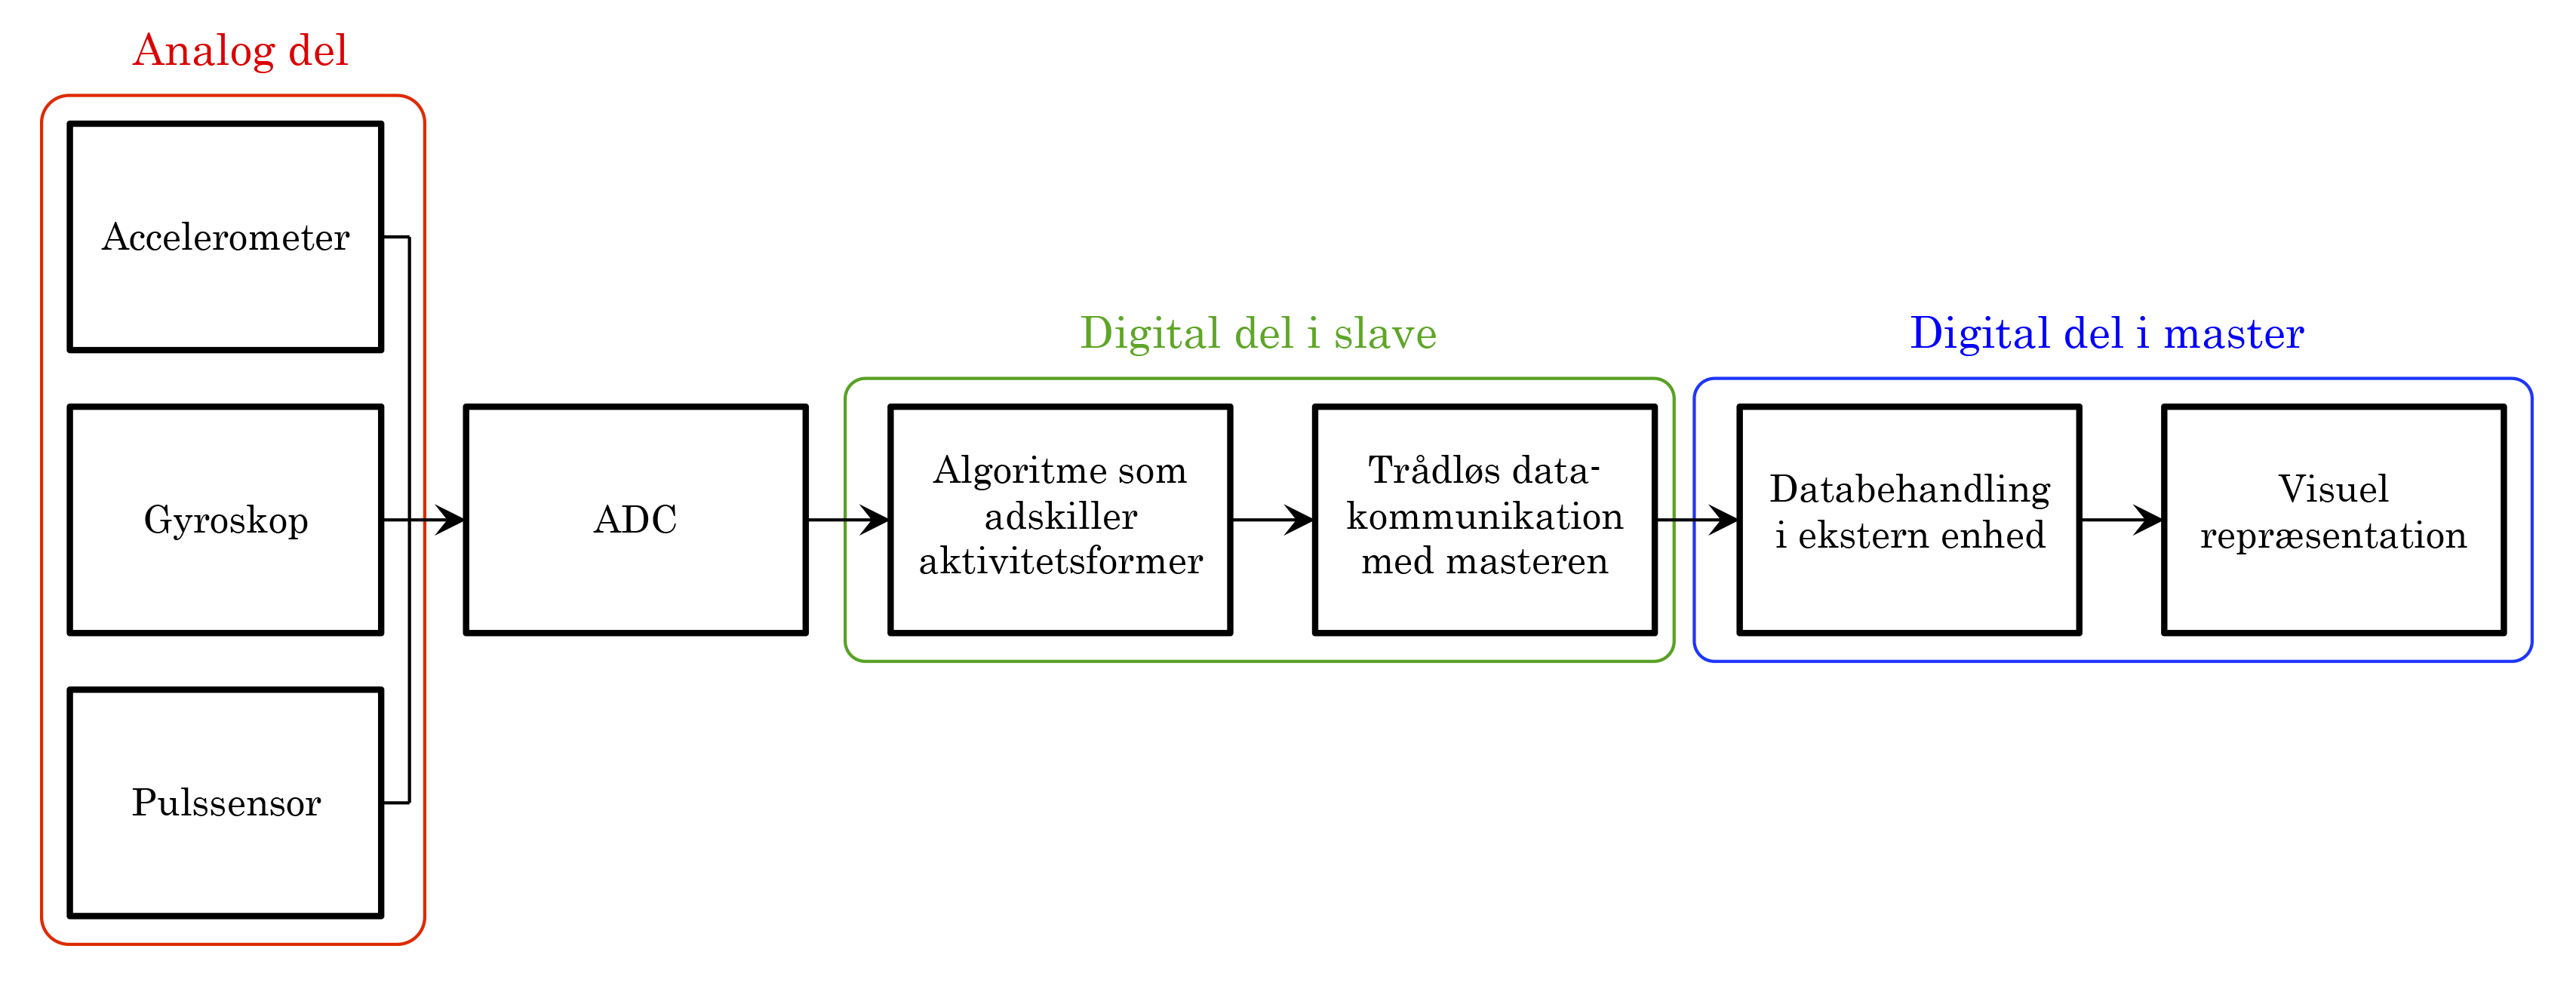
\includegraphics[scale=0.54]{figures/bProblemloesning/blokdiagram2.png}
 	\caption{Blokdiagram for systemet, som opdeles i den analoge del, og de to digitale dele. Den analoge del er omkranset med en rød firkant, slaven er omkranset med en grøn firkant og master er omkranset med en blå firkant.}
 	\label{fig:blokdiagram}
 \end{figure}
\section{Brugersikkerhed}
\textit{Nedenstående afsnit beskriver hvilke ricisi der kan forekomme når en bruger tilkobles elektronisk udstyr. Metoder hvorpå de omtalte risici kan forebygges, beskrives også. Afsnittet underbygges af det funktionelle krav, hermed at systemet skal været sikkert for brugeren at anvende.}

Medikoteknisk udstyr er tilsluttet en spændingsforsyning i form af eksempelvis strømnettet eller et batteri. Der indgår derfor en spænding og dermed en elektrisk strøm i det elektroniske kredsløb. En elektrisk fare kan opstå når brugeren er tilkoblet det medikotekniske udstyr, og kan dermed risikere at blive udsat for makro- og mikroshock fra hele det elektriske kredsløb. Makroshock er defineret som en elektrisk strøm, som løber igennem kroppen på den tilsluttede person. Denne strøm løber oven på huden, og er overfladisk. Mikroshock er defineret som elektrisk strøm, som løber igennem en persons væv deriblandt hjertet. Den elektriske strøm som personen påvirkes med under mikroshock, medfører oftest en større potentiel fare end makroshock. Eksempelvis kan makroshock forårsage mindre muskelkontraktioner og er ofte ikke-dødelige skader. Derimod kan mirkoshock være store vævsskader samt dødelige elektriske påvirkninger af personen. \citep{Webster2011} \newline
Medikoteknisk udstyr har dermed en risiko for at påføre brugeren en strøm som potentielt kan være farlig. Det er derfor væsentligt, at det elektroniske udstyr involverer sikkerhedsmæssige elementer således risikoen for lækstrømme sænkes. Eksempelvis benyttes isolation og jordning som sikkerhedsmæssige procedurer, for at nedbringe risikoen for at tilføre brugeren lækstrømme i form af henholdsvis makroshock eller mikroshock. Isolation benyttes til at isolere brugeren fra elektriske spændingskilder i det medikotekniske udstyr. Ydermere benyttes jording som en sikkerhedsforanstaltning, idet alle aktive komponenter føres til jord, altså et fælles nulpunkt. De aktive komponenter er forbundet til jord, hvormed eventuelle lækstrømme vil løbe denne vej og dermed væk fra brugeren. \citep{Webster2011} \newline 
Systemet skal være mobilt som det fremgår af \secref{succeskrav}. Systemet vil dermed have en spændingsforsyning i form af et knapcelle batteri, hvilket vil tilføre en lav spænding. Benyttelsen af batterier kan dog være forbundet med enkelte, mindre sikkerhedsmæssige farer. Farerne kan opstå hvis batterierne ikke bliver brugt efter de foreskrevne regler for det pågældende batteri. Dette kan risikere at ødelægge batteriet, hvormed brugeren vil kunne blive udsat for forbrændinger som følge af fejlbrug af batteriet. Et ødelagt batteri kan ydermere risikere at medføre åndedrætsbesvær for brugeren. Disse farer kan undgås hvis man følger batteriets sikkerhedsanvisninger. \citep{NREL2011}


%  For at sikre lækstrømme ikke opnår en størrelse hvormed makro- og mikroshock kan være alvorligt skadelige, kan isolation benyttes. Ved isolation sikre man at det medikotekniske udstyr ikke er i direkte forbindelse med en betydelig spændingskilde. I og med at udstyret er forsynet med en lav spændingskilde, begrænses størrelsen af de lækstrømme som kan forekomme. Den anden sikkerhedsforanstaltning som kan implementeres for at gøre udstyret sikkert for brugeren er jording. Jording sikre at alle

\begingroup
\raggedright
\bibliographystyle{unsrtnat}
\bibliography{kilder}
\endgroup

\begin{appendices}
	\chapter{Pilotforsøg}
\textit{Dette bilag beskriver pilotforsøget, som er nødvendigt i forhold til testmåling og design af aktivitetsmåleren. Der undersøges tre forskellige placeringer af sensoren i tre forskellige aktivitetsformer på fire forsøgspersoner.}

\section{Teori}

\section{Formål}
For at kunne modificere og tilpasse softwaren til CY8CKIT-043 PSoC 4 M-Series Prototyping Kit er det nødvendigt at vide, hvordan forskellige aktivitetsformer påvirker sensoren. Målingerne skal undersøges for at kunne lave en algoritme, som kan få sensoren til at skelne imellem de pågældende aktivitetsformer. Derudover skal det bestemmes, hvor sensoren skal placeres på kroppen for mest optimalt udbytte. Derfor er formålet med pilotforsøget at undersøge følgende:
\begin{itemize}
	\item Hvordan påvirkes sensoren af gang, løb og cykling? 
	\item Hvor mange g ændrer sensorens målinger sig alt efter placering på kroppen?
\end{itemize}

\section{Materiale}
\begin{itemize}
	\item Løbebånd med justerbar hastighed.
	\item Motionscykel.
	\item Shimmer3 sensor.
	\item Computer med Multi Shimmer Sync for Windows.
\end{itemize}

\section{Fremgangsmåde}

\subsection{Databehandling}

\section{Resultater}

\section{Diskussion}

\section{Konklusion}

Formål: 
Hvordan påvirker gang, løb og cykling sensorene? 
Kan man se forskel på dataene i forhold til hvilken bevægelse der udføres.
Lav et forsøg som starter med langsom gang og så bliver hurtigere og hurtigere løb - for at se om der sker en markant ændring når man skifter fra gang til løb (i forhold til eks. G)
Hvor stort et stød (G) er der alt efter hvor sensoren påsættes ved gang, løb og cykling?
Ankel, midt på skinnebenet, under knæet.


Fremgangsmåde
Forskellige hastigheder inden for det at gå og løbe 
^samme med cykling
Placering af sensorer

\end{appendices}


\end{document}